\documentclass[10pt]{article}
\usepackage{a4wide}
\usepackage[english]{babel}
\usepackage{graphicx}
\usepackage{tabu}
\usepackage{textcomp}
\usepackage{fancyhdr}
\usepackage{lastpage}
\usepackage{titlesec}
\usepackage{lscape}
\usepackage{longtable}
\usepackage{color}
\usepackage{listings}
\usepackage{xkeyval}
\usepackage{hyperref}

\definecolor{mygreen}{rgb}{0,0.6,0}
\definecolor{mygray}{rgb}{0.5,0.5,0.5}
\definecolor{mymauve}{rgb}{0.58,0,0.82}

\lstset{ % Syntax highliughting for java
    backgroundcolor=\color{white},   % choose the background color; you must add \usepackage{color} or \usepackage{xcolor}
    basicstyle=\footnotesize,        % the size of the fonts that are used for the code
    breakatwhitespace=false,         % sets if automatic breaks should only happen at whitespace
    breaklines=true,                 % sets automatic line breaking
    captionpos=b,                    % sets the caption-position to bottom
    commentstyle=\color{mygreen},    % comment style
    deletekeywords={...},            % if you want to delete keywords from the given language
    escapeinside={\%*}{*)},          % if you want to add LaTeX within your code
    extendedchars=true,              % lets you use non-ASCII characters; for 8-bits encodings only, does not work with UTF-8
    frame=none,                    % adds a frame around the code
    keepspaces=true,                 % keeps spaces in text, useful for keeping indentation of code (possibly needs columns=flexible)
    keywordstyle=\color{blue},       % keyword style
    language=Octave,                 % the language of the code
    morekeywords={*,...},            % if you want to add more keywords to the set
    numbers=left,                    % where to put the line-numbers; possible values are (none, left, right)
    numbersep=5pt,                   % how far the line-numbers are from the code
    numberstyle=\tiny\color{mygray}, % the style that is used for the line-numbers
    rulecolor=\color{black},         % if not set, the frame-color may be changed on line-breaks within not-black text (e.g. comments (green here))
    showspaces=false,                % show spaces everywhere adding particular underscores; it overrides 'showstringspaces'
    showstringspaces=false,          % underline spaces within strings only
    showtabs=false,                  % show tabs within strings adding particular underscores
    stepnumber=5,                    % the step between two line-numbers. If it's 1, each line will be numbered
    stringstyle=\color{mymauve},     % string literal style
    tabsize=4,                       % sets default tabsize to 2 spaces
    title=\lstname                   % show the filename of files included with \lstinputlisting; also try caption instead of title
}
%%%%%%
%% Variables for version and release status
%% useage: \version
%%%%%%
\newcommand\module{CS27020}
\newcommand\moduleName{Modeling Persistent Data}
\newcommand\authorText{Nicholas Dart}
\newcommand\authorUsername{nid21}
\newcommand\studentID{130057750}
\newcommand\assesser{Edel Sherrett}

%%%%%%
%% Alias
%%%%%%
%% \newcommand{\sectionbreak}{\clearpage}  %% Allways start a section on a new page


%%%%%%
%% Alias
%%%%%%
%\newcommand{\sectionbreak}{\clearpage}    %% Allways start a section on a new page
%% Never worked anyway...
%% ]\newcommand{\figureRef[x]{i}{d}{l}}{\begin{figure} \centering \includegraphics[scale=x]{i} \caption{d} \label{fig:l} \end{figure}}

\title{ \huge \module Assignment \\ \Large \moduleName}
\author{
    \vspace{100pt}
    \begin{tabular}{ r || l }
        Author          & \authorText (\authorUsername)\\
                        & \studentID \\
        Date Published  & \today \\
                        & \\
        Assessed By     & \assesser \\
        Department      & Computer Science \\
        Address         & Aberystwyth University \\
                        & Penglais Campas \\
                        & Ceredigion \\
                        & SY23 3DB \\
    \end{tabular} \\
    Copyright \textcopyright Aberystwyth University 2014
    %get rid of the date on the titlepage
    \date{}
}

\pagestyle{fancy}
\fancyhf{}
\lhead{\module~Assignment}
\rhead{\authorText~-~\studentID}
\rfoot{Page \thepage \hspace{1pt} of \pageref{LastPage}}
\lfoot{Aberystwyth University - Computer Science}

\begin{document}
    \setcounter{page}{1}

    \maketitle
    \thispagestyle{empty}
    \clearpage

    %\tableofcontents
    %\clearpage

    \section{Un-Normalized Data}

        \subsection{Structure Analysis}
            I have identified the following list of attributes that will be needed to be stored in the database:
            \begin{tabular} { | l | l | p{11cm} | }
                \hline
                Attribute Name & Likely Type & Comment \\ \hline
                Member Number & Int & Or User ID, This will probably be a primary or unique key for users \\ \hline
                Name & VarChar & Users First and Last Name. May want to split these into First Name and Last Name \\ \hline
                Phone & Text & Needs to be a Text to store leading zero \\ \hline
                Team Name & Text & \\ \hline
                Captain ID & Int & The UserID of the Team Captain \\ \hline
                Sport Name & Text & \\ \hline
                Training Time & Timestamp & Or some other Time/Date Format \\ \hline
            \end{tabular}

            These attributes will likely fall into three tables:

            \begin{itemize}
                \item Users - Holds a list of users; their ID's, Names and Phone numbers.
                \item Sports - Holds a list of Sports; their Names and Captain's Name and Phone number.
                \item Teams - Holds a list of Teams, their Players and training times.
            \end{itemize}

            I have inferred from the given diagram that a Sport can hold many teams, and that a team has a captain, a list of users and a list of training times.

            \subsection{Functional Dependencies}
                \begin{center}
                    \textbf{Member Number $\rightarrow$ Name, Phone}
                \end{center}
                Member Number will depend on a unique Name and a Unique Phone number, therefore for example if two people had the same phone number, but had unique names, they will receive a unique member number. This allows two people of the same first name to live in the same house and still be accepted by the system. There is however the (unlikely) possibility that two people will have the same first and last names, and provide the same phone number. However this will be rare, and can be minimized further if a middle name or other information is included.
                \begin{center}
                    \textbf{ Sport, Team $\rightarrow$ Captain }
                \end{center}

                A team can have only one captain, therefor a team name and a sports name will yield a captains details (name and phone). 

                \begin{center}
                    \textbf{Sport, Team $\rightarrow$ Players}
                \end{center}

                A list of players can be determined for a team given the name of the team and the name of the sport. This is to allow for teams with the same name to belong to different sports (eg Football and Rugby could each have a ``Team A''). The list of players will contain their names, phone numbers and member numbers.

        \section{Bottom-Up Analysis}
            
            \subsection{Iteration 1}
                Thus far the following tables have been presented in the diagram and example data:

                \begin{center}
                    \textbf{Users:}\\
                    \begin{tabular}{ | r | l | l | p{10cm} } 
                        \cline{1-3}
                        PK & UserID & Integer & \\ \cline{1-3}
                        & First Name & Text & \\ \cline{1-3}
                        & Last Name & Text & \\ \cline{1-3}
                        & Phone Number & Text & \\ \cline{1-3}
                    \end{tabular}
                \end{center}

                \begin{center}
                    \textbf{Sports:}\\
                    \begin{tabular}{ | r | l | l | p{10cm} } 
                        \cline{1-3}
                        & Sport Name & Text & \} Potentially Repeated Data \\ \cline{1-3}
                        & Team Name & Text & \} Potentially Repeated Data \\ \cline{1-3}
                        FK & Captain ID & Integer & \} Potentially Repeated Data \\ \cline{1-3}
                        FK & PlayerID & Integer & \} Potentially Repeated Data \\ \cline{1-3}
                        & Training Time & DateTime & \} Potentially Repeated Data \\ \cline{1-3}
                    \end{tabular}
                \end{center}

            \subsection{Iteration 2 - First Normal Form}

                All the fields in the Sports table can repeat; any user can be in any number of sports, with potentially any number of team. A User can also be a captain of any number of teams, and teams can have any number of training times. Therefor i propose a Players table to link a user to a sport:

                \begin{center}
                    \textbf{Users:}\\
                    \begin{tabular}{ | r | l | l | p{10cm} } 
                        \cline{1-3}
                        PK & UserID & Integer & \\ \cline{1-3}
                        & First Name & Text & \\ \cline{1-3}
                        & Last Name & Text & \\ \cline{1-3}
                        & Phone Number & Text & \\ \cline{1-3}
                    \end{tabular}
                \end{center}

                \begin{center}
                    \textbf{Sports:}\\
                    \begin{tabular}{ | r | l | l | p{10cm} } 
                        \cline{1-3}
                        PK & Sport ID & Integer & \\ \cline{1-3}
                        & Sport Name & Text & \} Potentially Repeated Data \\ \cline{1-3}
                        & Team Name & Text & \} Potentially Repeated Data \\ \cline{1-3}
                        FK & Captain ID & Integer & \\ \cline{1-3}
                        & Training Time & DateTime & \} Potentially Repeated Data \\ \cline{1-3}
                    \end{tabular}
                \end{center}

                \begin{center}
                    \textbf{Players:}\\
                    \begin{tabular}{ | r | l | l | p{10cm} } 
                        \cline{1-3}
                        FK & Sport ID & Integer & \\ \cline{1-3}
                        FK & User ID & Integer & \\ \cline{1-3}
                    \end{tabular}
                \end{center}

                At this point, I believe my structure is in first normal form as there is no repeating data within a field; the definition is as such:
                \begin{quotation}
                    It states that the domain of an attribute must include only atomic (simple, indivisible) values and that the value of any attribute in a tuple must be a single value from the domain of that attribute.
                    \begin{flushright}
                        -- Elmasri, Ramez and Navathe, Shamkant B. (July 2003).\\
                        Fundamentals of Database Systems, Fourth Edition. Pearson. p. 315
                    \end{flushright}
                \end{quotation}


            \subsection{Iteration 3 - Second Normal Form}

                To Achieve 2NF, Sports and teams must be separated, this then leads to problems relating a user to a sport, without specifying a team. Therefor a table relating a user to a sport should be used, with another table relating a sport-playing-user to a team.

                \begin{center}
                    \textbf{Users:}\\
                    \begin{tabular}{ | r | l | l | p{10cm} } 
                        \cline{1-3}
                        PK & UserID & Integer & \\ \cline{1-3}
                        & First Name & Text & \\ \cline{1-3}
                        & Last Name & Text & \\ \cline{1-3}
                        & Phone Number & Text & \\ \cline{1-3}
                    \end{tabular}
                \end{center}

                \begin{center}
                    \textbf{Sports:}\\
                    \begin{tabular}{ | r | l | l | p{10cm} } 
                        \cline{1-3}
                        PK & Sport ID & Integer & \\ \cline{1-3}
                        & Sport Name & Text & \\ \cline{1-3}
                    \end{tabular}
                \end{center}

                \begin{center}
                    \textbf{Teams:}
                    \begin{tabular}{ | r | l | l | p{10cm} } 
                        \cline{1-3}
                        PK & Team ID & Integer & \\ \cline{1-3}
                        & Team Name & Text & \\ \cline{1-3}
                        FK & Sport ID & Integer & \\ \cline{1-3}
                        FK & Captain ID & Integer & \\ \cline{1-3}
                    \end{tabular}
                \end{center}

                \begin{center}
                    \textbf{SportingPlayers:}
                    \begin{tabular}{ | r | l | l | p{10cm} } 
                        \cline{1-3}
                        PK & SportsPlayer ID & Integer & \\ \cline{1-3}
                        FK & Player ID & Integer & \\ \cline{1-3}
                        FK & Sport ID & Integer & \\ \cline{1-3}
                    \end{tabular}
                \end{center}

                \begin{center}
                    \textbf{TeamPlayers:}
                    \begin{tabular}{ | r | l | l | p{10cm} } 
                        \cline{1-3}
                        FK & SportsPlayer ID & Integer & \\ \cline{1-3}
                        FK & Team ID & Integer & \\ \cline{1-3}
                    \end{tabular}
                \end{center}

                \begin{center}
                    \textbf{Training Times:}
                    \begin{tabular}{ | r | l | l | p{10cm} }
                        \cline{1-3}
                        FK & Team ID & Integer & \\ \cline{1-3}
                        & Training Time & DateTime & \\ \cline{1-3}
                    \end{tabular}
                \end{center}

            \subsection{Iteration 4 - Third Normal Form}

                For third normal form, I seperated out day of the week (in accordance to RFC5545 \url{https://tools.ietf.org/html/rfc5545#page-37})

                \begin{center}
                    \textbf{Users:}\\
                    \begin{tabular}{ | r | l | l | p{10cm} } 
                        \cline{1-3}
                        PK & UserID & Integer & \\ \cline{1-3}
                        & First Name & Text & \\ \cline{1-3}
                        & Last Name & Text & \\ \cline{1-3}
                        & Phone Number & Text & \\ \cline{1-3}
                    \end{tabular}
                \end{center}

                \begin{center}
                    \textbf{Sports:}\\
                    \begin{tabular}{ | r | l | l | p{10cm} } 
                        \cline{1-3}
                        PK & Sport ID & Integer & \\ \cline{1-3}
                        & Sport Name & Text & \\ \cline{1-3}
                    \end{tabular}
                \end{center}

                \begin{center}
                    \textbf{Teams:}
                    \begin{tabular}{ | r | l | l | p{10cm} } 
                        \cline{1-3}
                        PK & Team ID & Integer & \\ \cline{1-3}
                        & Team Name & Text & \\ \cline{1-3}
                        FK & Sport ID & Integer & \\ \cline{1-3}
                        FK & Captain ID & Integer & \\ \cline{1-3}
                    \end{tabular}
                \end{center}

                \begin{center}
                    \textbf{SportingPlayers:}
                    \begin{tabular}{ | r | l | l | p{10cm} } 
                        \cline{1-3}
                        PK & SportsPlayer ID & Integer & \\ \cline{1-3}
                        FK & Player ID & Integer & \\ \cline{1-3}
                        FK & Sport ID & Integer & \\ \cline{1-3}
                    \end{tabular}
                \end{center}

                \begin{center}
                    \textbf{TeamPlayers:}
                    \begin{tabular}{ | r | l | l | p{10cm} } 
                        \cline{1-3}
                        FK & SportsPlayer ID & Integer & \\ \cline{1-3}
                        FK & Team ID & Integer & \\ \cline{1-3}
                    \end{tabular}
                \end{center}

                \begin{center}
                    \textbf{Training Times:}
                    \begin{tabular}{ | r | l | l | p{10cm} }
                        \cline{1-3}
                        PK & Time & Time & \\ \cline{1-3}
                        FK & Day & Character(2) & \\ \cline{1-3}
                    \end{tabular}
                \end{center}

                \begin{center}
                    \textbf{Day:}
                    \begin{tabular}{ | r | l | l | p{10cm} }
                        \cline{1-3}
                        PK & Day & Character(2) & \\ \cline{1-3}
                    \end{tabular}
                \end{center}

        \section{Postgresql}
            \subsection{Creation query}
                \lstinputlisting[language=sql]{PSQL-schema.sql}

            \subsection{Insertion}
                \lstinputlisting[language=sql]{insertion.sql}

            \subsection{Selection Queries}
                \lstinputlisting[language=sql]{querys.sql}
                    
        \begin{landscape}
            \section{Screenshots}
                \subsection{Creation Query}
                    \begin{center}
                        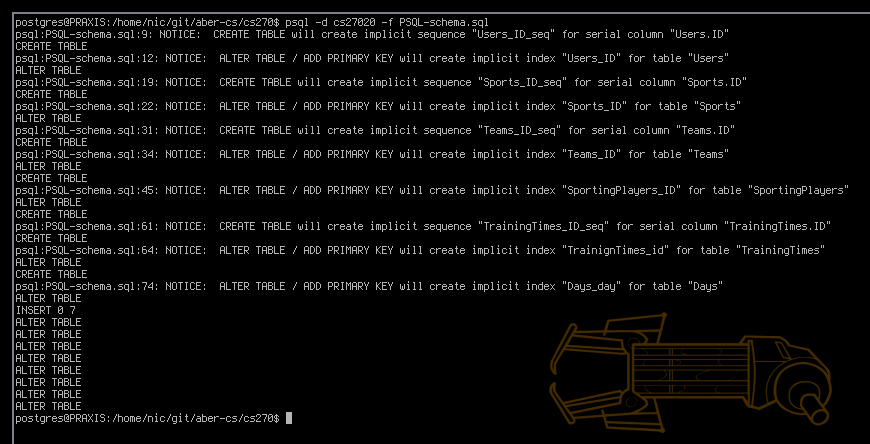
\includegraphics[scale=0.75]{createQuery_cropped.png}
                    \end{center}
        \end{landscape}
            \subsection{Selection Query}
                \begin{center}
                    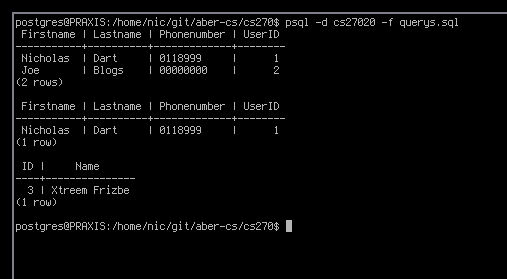
\includegraphics[scale=0.75]{selectionQuery_cropped.png}
                \end{center}

\end{document}